% ============================================================================
% CHAPTER 8 — DL AUTOENCODERS FOR COHERENT OPTICAL OFDM
% ============================================================================
\chapter{DL Autoencoders for Coherent Optical OFDM Systems}
\label{ch:dl_ae_optical}

\begin{motivation}
    The ESLM-AE of Chapter~\ref{ch:eslm_ae} addressed optical OFDM with
    intensity modulation (DCO-OFDM, VLC).  But what about
    \textbf{Coherent Optical OFDM (CO-OFDM)}, the dominant modulation
    format in long-haul fiber-optic communications?
    CO-OFDM uses complex-valued signals (like RF OFDM) rather than
    real-valued intensity signals, and the channel is a dispersive
    optical fiber rather than a wireless link.
    Alnaseri et al.\ (2025) adapted the autoencoder approach to CO-OFDM,
    demonstrating that learning-based PAPR reduction is effective even
    in the demanding optical fiber environment~\cite{alnaseri2025deep}.
\end{motivation}


% ----------------------------------------------------------------------------
\section{Conceptual Overview}
\label{sec:dlae_concept}
% ----------------------------------------------------------------------------

CO-OFDM combines the spectral efficiency of OFDM with the coherent detection
capability of optical receivers, enabling high-capacity long-haul
transmission.  However, CO-OFDM suffers from the same high-PAPR problem
as RF OFDM, with the additional complication that fiber nonlinearity
(Kerr effect) makes the system even more sensitive to peak power
than wireless systems~\cite{alnaseri2025deep}.

The DL-AE approach treats the CO-OFDM transmitter and receiver as a
single autoencoder trained to minimize both PAPR and reconstruction
error.  The key difference from PRNet is the \textbf{channel model}:
instead of simple AWGN, the optical fiber channel includes chromatic
dispersion, polarization mode dispersion, and nonlinear
effects~\cite{alnaseri2025deep}.


% ----------------------------------------------------------------------------
\section{System Model and Architecture}
\label{sec:dlae_architecture}
% ----------------------------------------------------------------------------

\begin{figure}[H]
    \centering
    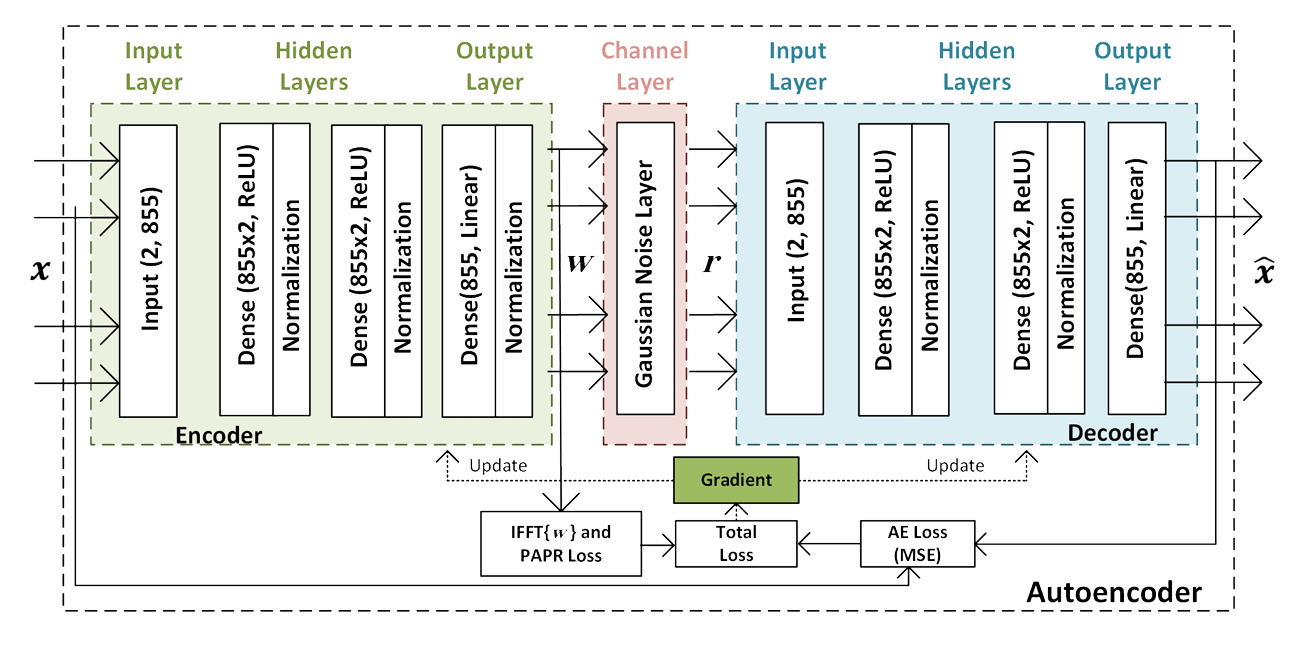
\includegraphics[width=0.95\linewidth]{Figures/44_dl_ae_structure.png}
    \caption{Autoencoder structure for CO-OFDM.  The encoder transforms
             the frequency-domain data into a low-PAPR time-domain signal.
             The decoder reconstructs the original data from the received
             signal after fiber propagation.
             Reproduced from~\cite{alnaseri2025deep}.}
    \label{fig:dlae_structure}
\end{figure}

\begin{figure}[H]
    \centering
    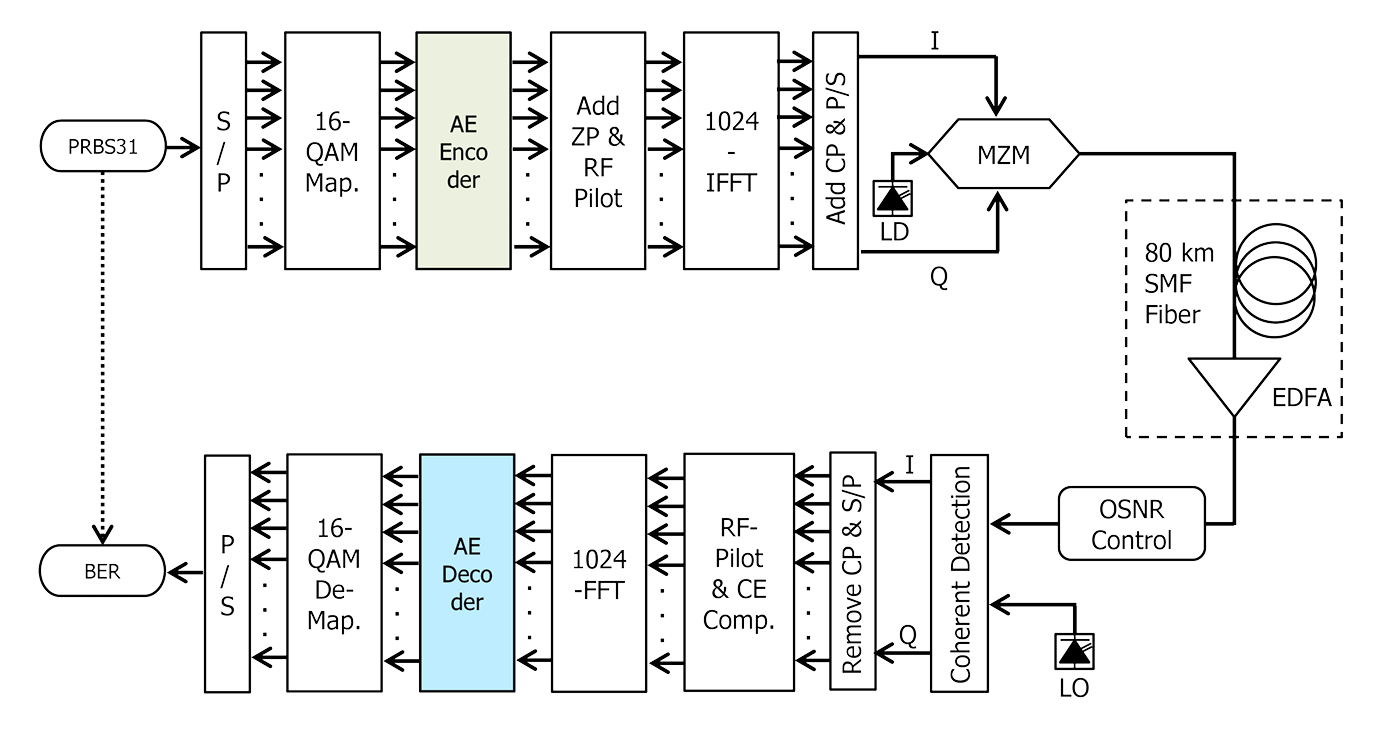
\includegraphics[width=0.95\linewidth]{Figures/45_dl_ae_co_ofdm.png}
    \caption{Complete CO-OFDM system with the autoencoder.
             The system includes the optical modulator, fiber channel
             (with dispersion and noise), coherent receiver, and
             the trained decoder.
             Reproduced from~\cite{alnaseri2025deep}.}
    \label{fig:dlae_system}
\end{figure}

\subsection{Encoder Architecture}

The encoder takes the real-valued representation of complex frequency-domain
data ($2N$ inputs) and produces a $2N$-dimensional output representing the
time-domain signal.  The architecture consists of fully connected layers
with ReLU activation and Batch Normalization~\cite{alnaseri2025deep}:
\begin{equation}
    \bm{s} = \mathcal{E}\!\bigl(\bm{X}_{\mathrm{real}};\;\bm{\theta}_E\bigr),
    \label{eq:dlae_encoder}
\end{equation}
where $\bm{X}_{\mathrm{real}} = [\Re(\bm{X})^T,\; \Im(\bm{X})^T]^T$
is the $2N$-dimensional real representation.

\subsection{Decoder Architecture}

The decoder mirrors the encoder and recovers the data from the received
signal after the optical channel~\cite{alnaseri2025deep}:
\begin{equation}
    \hat{\bm{X}}_{\mathrm{real}}
    = \mathcal{D}\!\bigl(\bm{r}_{\mathrm{real}};\;\bm{\theta}_D\bigr).
    \label{eq:dlae_decoder}
\end{equation}


% ----------------------------------------------------------------------------
\section{Training Procedure}
\label{sec:dlae_training}
% ----------------------------------------------------------------------------

\subsection{Loss Function}

The loss function combines PAPR reduction with signal fidelity, analogous
to PRNet but adapted for the optical domain~\cite{alnaseri2025deep}:
\begin{equation}
    \mathcal{L}_{\mathrm{DL\text{-}AE}}
    = \gamma \cdot \mathcal{L}_{\mathrm{PAPR}}(\bm{s})
    + (1 - \gamma) \cdot \mathcal{L}_{\mathrm{MSE}}(\bm{X},\, \hat{\bm{X}}),
    \label{eq:dlae_loss}
\end{equation}
where $\gamma$ is the PAPR-fidelity balance factor.


% ----------------------------------------------------------------------------
\section{Simulation and System Parameters}
\label{sec:dlae_params}
% ----------------------------------------------------------------------------

\begin{table}[H]
    \centering
    \caption{Simulation parameters for DL-AE CO-OFDM~\cite{alnaseri2025deep}.}
    \label{tab:dlae_params}
    \begin{tabular}{@{} l l @{}}
        \toprule
        \textbf{Parameter} & \textbf{Value} \\
        \midrule
        Number of subcarriers ($N$) & 1024 (855 data symbols) \\
        Modulation scheme & 16-QAM \\
        OFDM type & CO-OFDM \\
        Channel model & Optical fiber (dispersion + AWGN) \\
        Fiber length & 800 km (10 spans of 80 km) \\
        Encoder layers & 2 hidden layers \\
        Decoder layers & 2 hidden layers \\
        Neurons per layer & 855 \\
        Activation & ReLU (hidden), Linear (output) \\
        Batch Normalization & Yes \\
        Optimizer & Adam \\
        Learning rate & $10^{-3}$ \\
        Training SNR & 20~dB \\
        Training set size & $10^5$ symbols \\
        Epochs & 200 \\
        Batch size & 256 \\
        \bottomrule
    \end{tabular}
\end{table}


% ----------------------------------------------------------------------------
\section{Results and Analysis}
\label{sec:dlae_results}
% ----------------------------------------------------------------------------

\subsection{PAPR Reduction}

\begin{figure}[H]
    \centering
    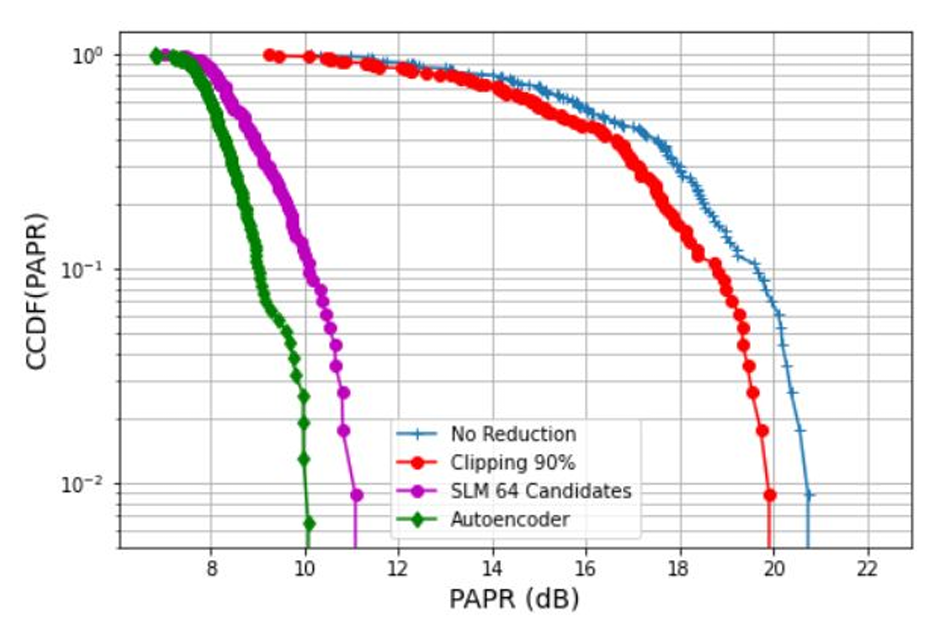
\includegraphics[width=0.65\linewidth]{Figures/46_dl_ae_ccdf.png}
    \caption{CCDF of PAPR for the DL-AE approach compared to
             conventional CO-OFDM and clipping.
             The autoencoder achieves significant PAPR reduction while
             avoiding the distortion introduced by clipping.
             Reproduced from~\cite{alnaseri2025deep}.}
    \label{fig:dlae_ccdf}
\end{figure}

\subsection{BER Performance}

\begin{figure}[H]
    \centering
    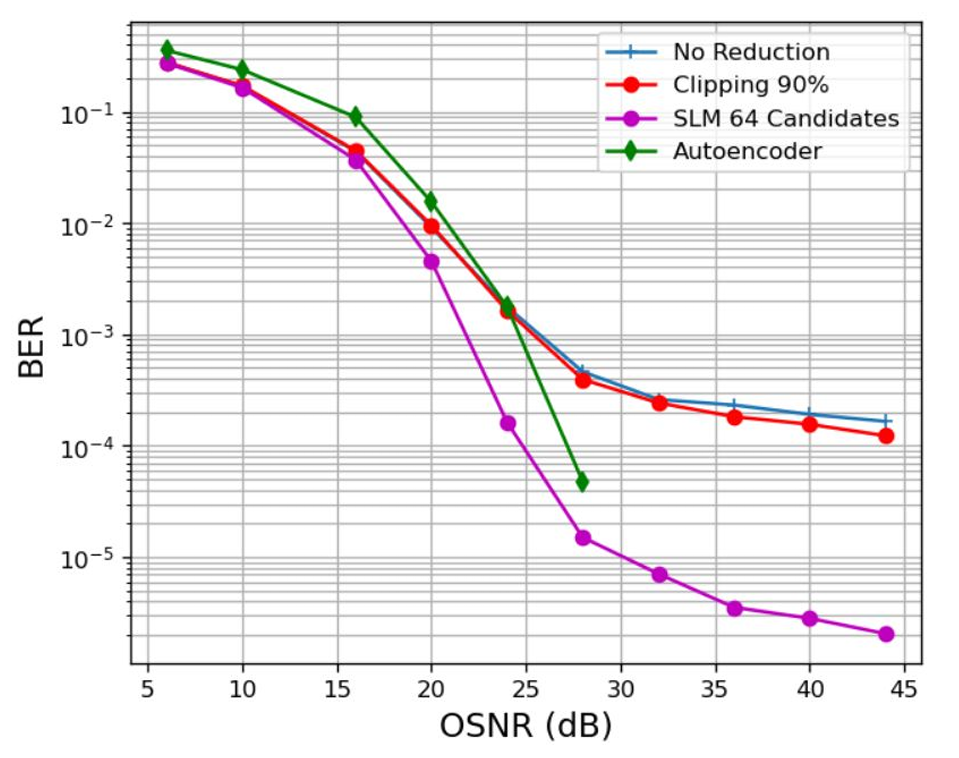
\includegraphics[width=0.65\linewidth]{Figures/47_dl_ae_ber_osnr.png}
    \caption{BER vs.\ optical SNR (OSNR) for the DL-AE CO-OFDM system.
             The autoencoder maintains acceptable BER across a range of OSNR
             values, demonstrating that the learned encoding is robust
             to optical channel impairments.
             Reproduced from~\cite{alnaseri2025deep}.}
    \label{fig:dlae_ber}
\end{figure}

\subsection{Effect of Noise Standard Deviation}

\begin{figure}[H]
    \centering
    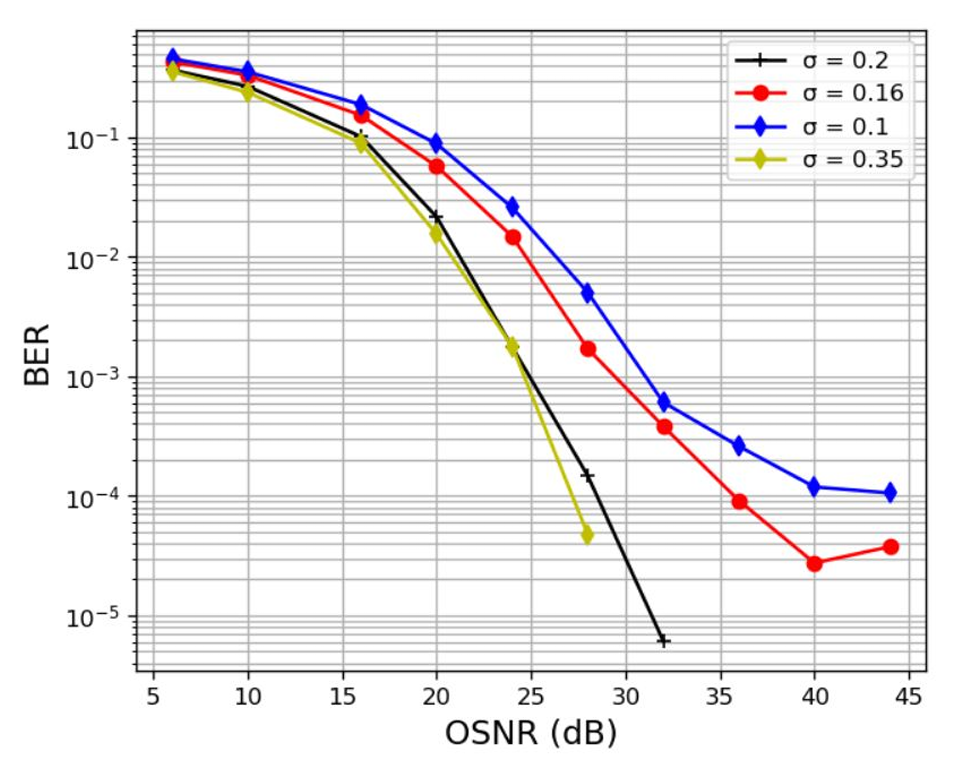
\includegraphics[width=0.65\linewidth]{Figures/48_dl_ae_ber_noise.png}
    \caption{BER vs.\ OSNR for the autoencoder learning with different noise
             standard deviations $\sigma$. The model achieves error-free 
             transmission when $\sigma$ is adequately modeled.
             Reproduced from~\cite{alnaseri2025deep}.}
    \label{fig:dlae_ber_noise}
\end{figure}

\begin{keyinsight}
    By exposing the autoencoder to varying levels of Gaussian noise
    during the forward pass training, the decoder learns to implicitly
    equalize and correct for both noise and nonlinear distortions over
    the fiber link, showcasing the major advantage of end-to-end
    learning~\cite{alnaseri2025deep}.
\end{keyinsight}


% ----------------------------------------------------------------------------
\section{Common Misconceptions}
\label{sec:dlae_misconceptions}
% ----------------------------------------------------------------------------

\begin{misconception}
    \textbf{``DL-AE for CO-OFDM is the same as ESLM-AE for DCO-OFDM.''} \\
    Despite both using autoencoders, these are fundamentally different:
    \begin{itemize}
        \item \textbf{Signal type:} CO-OFDM uses complex-valued signals
              (no Hermitian symmetry constraint); DCO-OFDM uses real-valued
              intensity signals.
        \item \textbf{Channel:} CO-OFDM operates over optical fiber
              (dispersion + Kerr nonlinearity); DCO-OFDM operates over
              a VLC channel (LED nonlinearity + multipath).
        \item \textbf{Architecture:} ESLM-AE generates phase factors within
              the SLM framework; the DL-AE learns a direct mapping
              (more like PRNet).
    \end{itemize}
    The autoencoder \emph{concept} is shared, but the implementations are
    tailored to their respective domains~\cite{alnaseri2025deep,hao2019extended}.
\end{misconception}


% ----------------------------------------------------------------------------
\section{Limitations and Open Problems}
\label{sec:dlae_limitations}
% ----------------------------------------------------------------------------

\begin{enumerate}
    \item \textbf{Simplified fiber model:}
          The simulations use a simplified optical channel model.
          Real fiber networks include polarization effects, amplifier
          chains, wavelength-division multiplexing crosstalk, and
          other impairments not captured~\cite{alnaseri2025deep}.

    \item \textbf{Fixed configuration:}
          Like PRNet, the network is tied to specific $N$ and modulation
          parameters.  Changing the system configuration requires retraining.

    \item \textbf{Moderate subcarrier count:}
          $N=64$ is small compared to practical CO-OFDM systems,
          which may use 256 or more subcarriers.

    \item \textbf{No explicit SLM connection:}
          The approach is a direct signal transformation, not linked to
          the SLM phase-rotation framework.
\end{enumerate}


% ----------------------------------------------------------------------------
\section{Connection to Other Approaches}
\label{sec:dlae_connections}
% ----------------------------------------------------------------------------

The DL-AE for CO-OFDM completes the autoencoder ``family'' in our document:
\begin{itemize}
    \item \textbf{PRNet} (Chapter~\ref{ch:prnet}): original autoencoder for
          RF OFDM (AWGN channel)~\cite{kim2017novel}.
    \item \textbf{ESLM-AE} (Chapter~\ref{ch:eslm_ae}): autoencoder +
          SLM structure for DCO-OFDM (VLC channel)~\cite{hao2019extended}.
    \item \textbf{DL-AE} (this chapter): autoencoder for CO-OFDM
          (optical fiber channel)~\cite{alnaseri2025deep}.
\end{itemize}

Each extends the autoencoder paradigm to a new domain and channel type,
demonstrating the versatility of the approach.

With all six ML-enhanced approaches now thoroughly examined, the next
chapter presents a systematic \emph{comparative analysis} of all methods
side-by-side~(Chapter~\ref{ch:comparative}).
